\chapter{绪论}{Introduction}
\label{chap:intro}

从人工智能发展的早期开始,实现人机之间的自然语言交互一直是该领域的研究焦点,1950年,Alan Turing提出了一个如何判定机器是否具有智能的标准“图灵测试”。至此,对话系统更是成为判定机器是否智能的理想模型。然而,对话系统一直是自然语言处理和人工智能领域的研究难题,它不仅涉及到对自然语言的处理,自然的对话系统还要求机器具备一定的认知能力,使其能按照人的响应方式与人类进行交互。本文从目前对话系统研究中亟待解决的认知技术角度出发,对此展开深入研究。

本章简要介绍智能对话系统的研究背景和意义、以及相关的研究现状和存在的问题,最后列出本文的主要研究内容和组织结构。

%%%%%%%%%%%%%%%%%%%%%%%%%%%%%%%%%%%%%%%%%%%%%%%%%%%%%%%%%%%%%%%
\section{研究背景和意义}{Background}
%%%%%%%%%%%%%%%%%%%%%%%%%%%%%%%%%%%%%%%%%%%%%%%%%%%%%%%%%%%%%%%  

      与机器进行智能对话一直是人们梦寐以求的梦想。随着人工智能技术的不断发展,对话系统逐渐成为人工智能在商业领域的焦点,各大公司也都纷纷高调发布对话系统产品,如在Jeopardy节目中夺冠的IBM Waston,苹果的Siri,微软的Cortana和小冰,小i和图灵等等。尽管近年来,对话系统相关的计算语言学和人工智能领域的很多技术都取得了巨大的进展,如语音识别和合成、机器翻译、信息检索、浅层语义分析甚至情感分析等,但对话系统的认知对话管理和语义语用等深层理解领域仍没有根本性的突破。即使是目前表现最好的对话系统,也依然是基于表层的语言分析和简单的启发性知识来实现。然而如果对话系统无法作为一个认知主体,以拟人的方式去感知和交互,就很难激发人类与其长时间交流的兴趣。
   
       对话系统涉及的领域很广,本文重点考虑认知型的对话系统,也就是强调机器作为一个认知主体,去理解和适应人的交流方式,从而使用户能用与人交流的自然方式去和机器交流。本文中提到的对话系统中的相关认知技术主要包括知识的深层表示、不确定性逻辑推理、语言与涉身知识的融合以及动机驱动的对话控制。对这些领域的研究显然具有重要的研究价值。这些领域中任一组块取得进展,不仅仅对于智能对话系统,而且对于其他领域,如语义理解、情感建模、自动化学习系统等等,都会有相当大的辅助和促进作用。另一方面,对话系统中的认知技术得到改进,无疑能大幅度提高对话系统的实用价值。能帮助机器更好更准确地结合语境理解和适应用户的交流方式,从而更准确更人性化地帮助人类完成一系列的辅助工作,拟人的交流方式也会使人们觉得更舒心和信赖,这也将为人们的生活带来诸多便利。

         尽管拥有巨大的研究价值和市场价值,研究者也发现构建一个能达到人类水平的对话系统是一项十分艰巨的任务。本文的研究着重于对话系统中的相关认知技术,提出了一个动机驱动的对话控制模型,即结合了心理学上的动机驱动模型,言语行为理论,以及基于概率逻辑网络的超图形式的知识表示,赋予对话系统一定的认知能力,从而使机器能作为一个认知主体,以更自然的方式与用户进行交互。

%%%%%%%%%%%%%%%%%%%%%%%%%%%%%%%%%%%%%%%%%%%%%%%%%%%%%%%%%%%%%%%
\section{研究现状综述}{The State of the Arts}
\label{sec:review}
%%%%%%%%%%%%%%%%%%%%%%%%%%%%%%%%%%%%%%%%%%%%%%%%%%%%%%%%%%%%%%%

对话系统简单来说就是计算机用来试图和人类通过自然语言交流的软件系统。对话系统的思想可以追溯到1950年图灵在\cite{Turing1950}中提出的图灵测试,在过去的几十年中,有关对话系统的研究大致有两个不同的方向:一个是仅在表面外观上模拟对话,也被称为聊天机器人,如著名的聊天机器人心理医生ELIZA\cite{Weizenbaum1966}等。这类系统大多数不考虑理解对话内容的含义,直接采用模板匹配的方式找到和用户输入相关的对话,目前经常被用在各类社交网站和实时通讯的社交软件中。另一个是试图模拟人类真实的对话,并动态产生合适的对话,也被称为对话管理。后者是本文的研究重点,因此这一小节我们将回顾这一类对话系统以及对话管理的相关研究。

目前,对话系统的研究中有很多不同的架构体系,一个对话系统包含哪些功能模块也视不同的系统而异,但一般来说,对话系统主要包括以下几个功能模块:自然语言理解模块、对话管理模块、知识表示模块、自然语言生成模块\cite{Arora2013}。各模块之间的数据走向如图\ref{fig:dialogue}所示。接下来我们将分别就对话系统中的各个功能模块来展开综述相关研究现状。另外,由于本文的智能对话系统中使用了言语行为理论的启发和指导,因此也会在本节对其相关研究进行简明的阐述。需要说明的是,本文研究的对话系统暂时只是基于文本的,所以这里暂且不讨论语音识别和语音合成模块。

\begin{figure}[htb]
\centering
\includegraphics[width=12cm]{figures/dialogue_system.png}
\caption{对话系统的基本结构}
\label{fig:dialogue}
\end{figure}


%%%%%%%%%%%%%%%%%%%%%%%%%%%%%%%%%%%%%%%%%%%%%%%%%%%%%%%%%%%%%%%
\subsection{知识表示及相关逻辑推理研究综述}{Overview of Knowledge Representation And Logic Reasoning}
\label{sec:representationReview}
%%%%%%%%%%%%%%%%%%%%%%%%%%%%%%%%%%%%%%%%%%%%%%%%%%%%%%%%%%%%%%%

对于任何以实现复杂功能为目标的自然语言处理系统(如对话系统或复杂的问答系统)来说,该系统内部的知识表示形式,即如何表示语义处理后的自然语言,往往是系统的各方面性能表现的关键所在。本小节将介绍知识表示目前的研究现状并回顾一些典型的知识表示方法及相应的优缺点,我们也会在本节重点介绍与本文所采用的知识表示相关联的几个具有代表性的知识库。

如何合理有效地表示自然语言话语的含义是过去50年来一直被争议的问题,这也是从一个句子中抽取信息的语义建模问题所面临的第一步。然而目前,“知识表示”需要满足哪些条件仍然处于争论状态。Jurasky和Martin在经典的《自然语言处理综论》\cite{Jurafsky2009}的第14章中从不同方面总结了一个完整的知识表示体系所要满足的计算需求,其中包括:

\begin{itemize}
\item 可能性验证(Verificability):必须能够确定知识表示的真实性,即知识表示体系能将输入的命题表示与储存相关知识的世界知识库中的表示相比较或匹配。
\item 无歧义表示(Unambiguous Representation):知识表示的语言支持的表示只能有一个无歧义的解释。
\item 规范形式(Canonical Form):表达同样信息的输入必须具有同样的知识表示形式,即规范形式。
\item 推论与变元(Inference and Variables):知识表示体系能根据输入的知识表示以及储存的背景知识推理出可靠结论。
\item 表达能力(Expressiveness):知识表示方法需要具备足够的表达能力来处理各种广泛领域的知识。
\end{itemize}

直到最近,这些需求列表一直被当做是知识表示领域中一个相当完善的黄金标准。Yarin等人\cite{Yarin2013}指出了这个必要条件列表并不完整,并指出了知识表示体系还需满足下列需求:

\begin{itemize}
\item 不确定性和内涵的表示
\item 能使用可行的方式来抽取话语的信息(即,从数据中抽取相关知识表示的算法的需求)  
\item 从话语中推理出相对应的情感和观点
\item 从不同命题中获取相关的不确定性
\item 不仅需要区分具有不同的意义的话语,还需区分涉及相似意义的话语
\item 在从话语中获取活动信息的同时还要获取活动相关的动作者(agent)
\item 回答问题除了使用相关的知识外,还需要能利用这些知识和问题的意义。
\item 对同一个意义,能生成不同表达方式的话语
\end{itemize}

当然这些需求本身也没有得到相关的验证是否就完全,但近几年提出的一些知识表示方法及相关研究也在试图满足这其中的部分或所有需求。下面我们将简单回顾一些具有代表性的知识表示方法以及相应的优缺点,从中也不难看出未来知识表示领域的研究方向。知识表示的任务比较繁琐,所涉及的领域比较广,因此很难有一个完整的分类体系来概括所有的知识表示方法,本文通过以下几方面来分类介绍典型的具有实用价值的知识表示方法。

\begin{enumerate}
\item {传统的知识表示方法}

这里的传统的知识表示方法主要指逻辑表示法、框架表示法以及语义网络表示法,以及在这基础上的一些延伸表示方法,下面将对这几类典型的传统知识表示方法做简单的分析和对比。

\begin{enumerate}
\item[1)] 逻辑表示法

逻辑表示法的思路是将自然语言话语转换成某种逻辑约束下的一组逻辑表达式,以及在该逻辑上对这些逻辑表达式的语义解释。常见的用于知识表示的逻辑有命题逻辑,传统逻辑以及谓词逻辑等。对复杂的自然语言来说,命题逻辑和传统逻辑的表达能力相对弱,这里主要介绍基于谓词逻辑的知识表示方法。

谓词逻辑表示法中既包括一阶逻辑也包括高阶逻辑(如多个量词)的表示,但从实用角度来看,也就是在有限数量信息的下,两者之间可以通过一定的逻辑等价推理来转换,而一阶逻辑具有简洁和易推理的优点,因此相对来说更广泛地被应用,也是被研究地相对成熟的一种知识表示方法。

基于一阶逻辑的知识表示体系中使用了三种基本构件:常量(有时也称为原子atom),函数以及变量,每一个构件都指向世界知识中的某个对象。其中,常量通常用于表示世界知识中的对象,比如“狗”;函数通常定义在常量或者变量上,在自然语言的背景下,“函数”可用于产生新的词汇。比如函数“Black(狗)”可生成“黑色的狗”或者“黑狗”;变量则允许我们表达对非具体对象的陈述或预测。将这三个简单的构件和存在量词以及连接符号和否定关系符号,我们可得出以下的表达式用于表示“存在一个实体,这个实体拥有一只黑色的狗,并且给这只黑色的狗喂了红色的肉。”

$$ 
\exists X(Own(X, Black(Dog))\land Feed(X, Black(Dog), Red(Meat))) 
$$


在上述的逻辑表达式上,我们可以进行相关的逻辑推理和蕴含等操作,并且能通过\lambda表达式来确定命题的真值。一阶逻辑表示法允许我们将自然语言话语表示成一种无歧义的表示方式。对于多义词,我们可以采用多个常量(原子)来表达,比如可以用$Bank_{institution}$来表示意思为“银行”的"Bank",用$Bank_{institution}$来表示意思为“河岸”的"Bank"。此外,这种表示方法的表达能力也适用于表达多个句子的情况。

比较典型的使用一阶逻辑的知识表示体系有早期的Cyc系统\cite{Lenat1990}。Cyc系统拥有一个非常丰富的人工编码知识库,它的终极目标是:以谓词逻辑的形式,将所有人类常识进行编码。虽然它的知识库中已存有数百万的谓词逻辑表达式,但到目前为止,似乎只对一小部分人类常识进行了编码。

一阶逻辑的知识表示方法相对简洁,但由于自然语言的复杂性和不确定性,如何将自然语言话语转换成一阶逻辑的表示形式,是一个极大的挑战。Pianatadosi等人\cite{Piantadosi2008}首先在几十个词的限定条件下构建一个概率模型,使其能对各种可能的语法建模并过滤掉过于复杂的,从而根据这些语法模型来得到相应的一阶逻辑表示形式。在此基础上,他们的研究还深入到通过递归方式来遍历所有可能的上下文无关文法的概率模型,使得递归进行到一定程度能得到一个对话语进行最佳解析的一阶逻辑表示形式。该方法最终能得到一个不可扩展的在迷你规模语法基础上的组合语义获取模型,并没有实用价值。

后期的Cyc系统也为了克服一阶逻辑表示方法的缺点,引入了贝叶斯网络来为该知识库中的概念和事件提供相应的概率真值,但后期Cyc系统也转入商业用途,其数据和表示也不免费公开,因此我们尚不清楚目前其具体研究状况。

\item[2)] 基于框架的知识表示法

基于框架的知识表示方法又被称为槽填充表示法。框架(Frame)可以理解成一种将某一对象或事件所涉及的知识信息存储在一起的复杂的数据结构,通常包括主体和槽(Slot)两部分,其中主体是固定的,表示一个特定的概念、对象或事件,而槽用于表示主体的各属性及属性值。其一般形式可以表示如下:

       <主体>  

       <槽名1><槽值1>| <侧面名11><侧面值111,侧面值112,…>

                                    <侧面名12><侧面值121,侧面值122,…>

比如“我吃蛋炒饭”可以表示成框架形式如下:

       <吃>  

       <施事者><我>

       <受事者><蛋炒饭>


基于框架的知识表示常被用于语义角色标注中,即标注出句子中的谓词以及相应的参数。比如“我吃蛋炒饭”,语义角色标注可以标注出其中谓词是“吃”(框架主体,表示事件),该事件的槽值可以表示为施事者“我”,受事者“蛋炒饭”。

基于框架的表示法具有代表性的系统有FrameNet\cite{Atkins1995}, FrameNet是一个人工编写的基于框架的语义知识库,其中包含了1,200个语义框架,13,000个词汇单元,大约19万个例句,目前被广泛用于语义角色标注的训练语料。

基于框架的表示形式也可以很容易被转换成等价的一阶逻辑表示形式。与一阶逻辑表示相似,将自然语言话语转换成基于框架的表示形式也是该表示方法的巨大挑战。

\item[3)] DCS树\cite{Liang2013}

鉴于将自然语言话语转换成上述两种表示形式非常困难,Liang等人\cite{Liang2013}试图将该任务简化成一个允许进行高效推理的约束满足的问题。为此,他们提出了一种新的知识表示方式:基于依存的组合语义树(Dependency based  Compositional Semantics Tree,以下简称DCS树),并通过预先设定的触发词和谓词的约束来高效地将自然语言转换成DCS树的表示形式,如单词city将会触发相应的谓词city。DCS树通过树的形式来构建逻辑表达式,它与依存句法树平行,为自然语言的语义解析提供了很多便捷。尽管该方法的提出只针对小规模数据集合上和预先设定的触发词表,但不难通过语义角色标注和浅层语义分析抽取出语句中的谓词等自动方法来代替这些人工编写的词汇表,从而扩大该方法的应用规模。此外,该表示方法还能结合大规模的事实数据库,如Freebase\cite{Bollacker2008},通过简单的语义角色标注和基于对先前观察的语句来填充语义空槽,从而实现对现有问答系统的扩展。


尽管DCS树的表达方式在有限领域和数据集合上能达到较好的效果,但从其研究\cite{Liang2011}来看,该表示方法的表达能力仍然是个悬而未决的问题,目前也没有任何相关研究表明其表达能力与一阶谓词逻辑的表示方法相当。从另一个角度来看,DCS树的表达方式受数据库查询语言的启发\cite{Yarin2013},通过数据库查询语言来表示自然语言语句的语义为知识表示提供了一个全新的思路,并不仅因为它将数据库查询语言的成熟研究也应用到语义表示和学习方面,而且它也实现了在约束满足条件下有效进行逻辑推理和蕴涵\cite{Giordani2010a}, \cite{Giordani2010b}, \cite{Giordani2009}。然而即使数据库查询语言相当成熟,但其表达能力仍然是非常有限的,因为这些语言除了无法表示聚合函数和相关的算术运算,还无法表达递归查询\cite{Libkin2003},但递归结构在自然语言中显然是相当常见的,这在一定程度上间接说明了DCS树的表达能力不一定足够用于实用的自然语言处理应用领域。

\item[4)] 语义网络表示法

语义网络的知识表示是人工智能和自然语言处理等领域的又一种经典的知识表示方式,它主要用于表示陈述性知识。语义网络在形式上是一个加权有向图,其中有向图的结点表示某个概念、对象、事件或状态等,边(也称为弧)则表示结点之间的语义关系。

语义网络中的语义关系通常包括实例关系(ISA,用于表示实体结点和类结点之间的关系,如“史努比”和“狗”)、泛化关系(AKO,用于表示类结点与抽象层次更高的类结点,如“鲸鱼”和“哺乳动物”)、部分整体关系(Part-of,用于表示结点与其组成成分之间的关系)以及属性值关系(用于表示个体的各属性和对应的属性值之间的关系,通常使用语义网络中的边来表示属性,用边所指向的结点来表示该属性的值)。除此之外,语义网络还能表示以谓词或关系为中心组织语义关系,还可表示不同子网络之间的逻辑关系,如析取、合取、否定和蕴涵等。

语义网络的知识表示体系所采用的推理机制主要有匹配和继承,继承一般通过匹配和搜索来实现。在问题求解时,可以根据问题的描述来构造一个语义网络片段,并在语义网络知识库中查找可以与该语义网络片段匹配的子网络,然后根据查找到的匹配来回答问题。

目前被广泛使用的基于语义网络的知识表示库有ConceptNet\cite{Liu2004}和谷歌的知识图谱等。语义网络非常符合人类的思维习惯,其表达方式自然、简洁,易于理解。表达能力方面,语义网络不仅可以表示事物的属性状态、行为动作、目标功能等,而且还能表示事物之间的关联,为人工智能和自然语言处理等相关系统提供了便捷的知识推理平台,但是语义网络也面临着诸多挑战,首先,语义网络的形式过于简单,很难表达相对复杂的关系类型,复杂关系的引入很容易增加语义网络的复杂度,从而使知识的储存和检索过程变得相当复杂,甚至难以实现。其次,语义网络中的语义关系查询和推理往往需要计算复杂度非常高的图算法,而且基于图的算法一般可扩展性差,这就直接导致,在知识库达到一定规模后,将面临着计算效率问题的挑战。最后,该表示方法还面临着严重的数据稀疏问题的挑战,对那些在语义网络中对外连接较少的实体,意味着涉及到它们的路径很少,这导致图算法对其相关路径查询和逻辑推理带来很大的难度。


上述的几种表示方法都可以看成是刚性表示方法,因为它们都无法在逻辑推理和蕴涵过程中处理非确定性。然而真实世界中大部分知识都是非确定性的,近年来也有将概率引入到这些传统的知识表示方法中,如\cite{Poon2009} 中将依存树转换成准概率逻辑形式,并使用了马尔科夫逻辑网络 \cite{Domingos2007}进行语义解析,这样一来,该方法既能进行逻辑推理和蕴涵,同时处理其中的不确定性。然而,该表示仅限于表达一些基本形式的语句,\cite{Titov2011}将上述工作中的表示继续简化,在马尔科夫逻辑网络中使用了Pitman-Yor随机过程来对谓词和变量之间的概率依存关系进行建模,使其更适用于简单的角色标注的形式。这些仅仅是在传统逻辑表示上引入了概率随机过程等,下面我们将简单介绍一些基于概率逻辑的知识表示方法。

\item {基于概率逻辑的知识表示法}

随着大数据技术的不断发展,不确定性的知识表示和管理在人工智能各领域越来越被重视起来,如上所述,基于概率逻辑的知识表示使得知识表示库能以认知概率形式来储存世界知识中的不确定性。因此,近年来,基于概率逻辑形式的知识表示方法不断涌现并广泛应用于各类学习系统中,如马尔科夫逻辑网(MLN),归纳逻辑编程(ILP),概率逻辑编程(PLP),贝叶斯逻辑编程(BLP),随机逻辑编程(SLP),随机关系模型(SRM),概率关系模型(PRM)等等。篇幅关系,我们这里只简单介绍和本文所使用的知识表示方法相似的几个典型的基于概率逻辑的表示方法。

      贝叶斯逻辑编程 (Bayesian Logic Programs,以下称BLP)\cite{Kersting2007}采用贝叶斯网络来表示知识,其中节点表示命题子句,它是众多“概率Prolog”中的一种。BLP可以用于表示任意带概率的Prolog形式的关系,并能通过逻辑推理来传播这些概率。BLP中维持了概率层次上的“直接因果影响”和逻辑层次上“间接推理”的同构关系,使得该结构中的概率和逻辑推理能达到一致,而无需借助棘手的混合模型。Puech\cite{Puech2003}对BLP的表达能力进行深入研究,并将其与SLP(Stochastic Logic Programs)的表达能力进行对比,其结果显示SLP能将同样的知识表示成BLP的一个子类。但BLP中的推理机制(即通过结构化的EM算法来查找BLP结构)却比SLP要简单的多,而SLP中的推理机制是被公认为非常困难的\cite{DaRaett2003}。然而,由于BLP依赖于Prolog,也继承了Prolog的不足之处,如依赖于特定的逻辑表达式归一化、缺少可扩展的推理机制等。
     
     马尔科夫逻辑网(Markov Logic Network,以下称MLN)最初由Domingos等人提出\cite{Domingos2007},MLN采用一阶谓词逻辑来表示实体之间的逻辑关系,采用马尔科夫网络形式的概率图模型来推理其中的概率分布。其基本思想是使一阶谓词逻辑中的硬性规则约束有所松弛,换句话说,当一个可能世界违反了其中某条规则,这个可能世界存在的概率很低,而并非直接设为0。MLN对每条规则都设定一定的权值,用来表示这条规则对可能世界的约束力,当一个规则的权值很大,那么违反该规则的可能世界存在的可能性就越低。MLN较好地结合了一阶逻辑和概率图模型的复杂性和不确定性表示,因此在该领域曾被广泛应用,如(Huynh and Mooney, 2008; Mihalkova, Huynh, and Mooney, 2007; Mihalkova and Mooney, 2007),其中也包括在NLP的一些领域上的应用,如实体抽取和语义关系抽取等。然而,由于在概率图模型中的推理复杂性,MLN近几年来慢慢失去了热度(Beltagy, Chau, Boleda, Garrette, Erk, and Mooney, 2013)。MLN假设整个网络都是基于一个概率分布的,这显然也不太合常理,而本文采用的PLN以及下面要介绍的NARS\cite{Wang2006}就刻意避开这样的假设。

     与传统的知识表示方法相比,上述的知识表示方法的有点在于能在逻辑中表示认知的不确定性,然而,这些这些表示结构都是离散的,无法用来推理句子之间的相似度。因此\cite{Brocheler2012}提出了PLP(Probabilistic Similarity Logic )来引入原子之间的距离衡量机制,但目前只能用于简单的不确定性逻辑推理中。本文的认知对话系统中所使用的概率逻辑网(Probabilistic Logic Network,以下称PLN)也有类似的地方,且能够将其他非语言渠道(如机器视觉感知)获得的相似度通过概率推理整合得到句子之间的相似度,并整合到其他的逻辑关系(如继承关系)中。

      Pei的NARS\cite{Wang2006}引擎运用了传统逻辑推理法,并引入了独特的数学理论来管理传统逻辑关系中的不确定性。但NARS是构建在经验的基础上,而不是基于模型轮语义。 在许多方面,我们所使用的PLN逻辑形式化体系与NARS有类似的地方,但也存在巨大差异。PLN在一套独特的数学理论基础上同时采用了传统逻辑和谓词逻辑,并且根据概率论和模糊数学理论来推导出不确定性真值的公式,而NARS的不确定性推理体系则基于原始的非逻辑形式。

     图\ref{fig:nars}展示了基本演绎推理、归纳推理和外展推理公式。这些公式是PLN和NARS共有的。在每个关系式右边的$<s,c>$表示“每个关系的强度和置信度”。PLN和NARS使用不同的公式,从那些前提中推导(优势、信息)结论的真值。有关PLN的知识表示和推理机制我们将在第2.3节中进一步介绍

\begin{figure}[htb]
\centering
\includegraphics[width=12cm]{figures/nars.png}
\caption{ NARS/PLN 传统逻辑中演绎推理、归纳推理和回溯推理的形式 }
\label{fig:nars}
\end{figure}


\end{enumerate}

\item  {组合分布式知识表示法}

 分布式表示方法被用于词汇语义学领域已超过40年\cite{Jurafsky2008},该方法对词汇使用连续表示,也就是说,在表示一个词汇时,同时将其相邻的词也表示在二进制向量中,比较典型的例子就是被广泛使用的词袋模型(bag-of-words model)。但是这类表示方法无法表示较复杂的知识,因此逐渐被组合分布式的表示方法所取代。

      Coecke, Sadrzadeh, and Clark (2010)提出了将连续分布表示方法和传统的组合表示方法结合起来用于知识表示,并使用张量积(tensor product)将信息从词汇层次带入到更高层次,然后使用线性函数将其映射到较低维度的句子空间中。Grefenstette (2013) 中指出该表示方法是可以用于表示非确定性的,还解释了其中的线性函数映射等同于非量化的一阶逻辑;但也证明了量化的一阶逻辑表示是无法通过线性函数映射得到的。因此,他在该文研究中引入了非线性映射用于获取量化的一阶逻辑表示。


组合的分布式知识表示方法还被用于语义建模领域中(Van de Cruys, Poibeau, and Korhonen, 2013; Hermann, Grefenstette, and Blunsom, 2013) 。它提供精确的表示,具有较好的表达能力,常被用于情感和角色标注方面的推理,而且能表示不确定性和句子的真值,目前该领域的研究主要集中于在句子空间中有效地进行语句的含义抽取和逻辑推理,但仍然有待深入研究。



\end{enumerate}


   本文采取了基于超图形式的知识表示Atomspace,并在该表示上使用了概率逻辑网络PLN进行知识推理和学习,这将在第二章中更详细地介绍。


%%%%%%%%%%%%%%%%%%%%%%%%%%%%%%%%%%%%%%%%%%%%%%%%%%%%%%%%%%%%%%%
\subsection{对话管理研究综述}{Overview of Dialogue Management}
%%%%%%%%%%%%%%%%%%%%%%%%%%%%%%%%%%%%%%%%%%%%%%%%%%%%%%%%%%%%%%%

对话管理,也称为对话控制,是决定一个对话系统在对话中说什么的关键。一般来说,对话系统首先利用自然语言处理模块将用户的输入转换成系统所使用的知识表示形式,即该系统所能理解的语义形式,而对话管理模块会结合当前的语境、对话历史以及自身的知识库等因素输出一个概念层次上的应答。最终,自然语言生成模块会对这些概念层次上的应答转换成自然语言输出。

对话管理模块在不同的对话系统中完成的任务是不同的,但其主要功能可以归纳为以下几个方面:

\begin{itemize}

\item 搜索和查询:根据当前的输入以及语篇上下文,在知识数据库中搜索查询和用户输入相关的知识或可能应答内容。
\item 询问:如果无法查询,针对某一问题,询问更多相关信息,直到能提交一个合适有效的查询。
\item 确认:当用户的输入无法被理解时,反复请求确认语焉不详的信息,使得用户输入的信息更具有操作性。
\item 预测:预测对话的进行方向。为对话系统的下一步操作即自然语言生成模块提供概念层次上的应答内容。
\item 控制:为了能实现自然流畅的类似人类的对话,采用一定的对话控制及交互策略,如:介入对话;回应惯用语;多方对话等。
\end{itemize}

在目前的研究现状下,对话管理模块在几乎所有目前存在的对话系统中起到了关键的作用。在实现方面,对话管理必须找到并返回能使对话保持与对话历史协调的最合适的响应。迄今为止,随着越来越多的相关研究和发展,对话管理的处理方法已经有很多,目前主流的对话管理方法可以分为三类:基于知识的对话管理;数据驱动的对话管理;基于混合方法的对话管理。下面会分别介绍这些对话管理方法的研究现状。

\begin{enumerate}

\item 基于知识的对话管理

早期的对话系统都是由具备特定领域知识的开发者来设计,如SUNDIAL\cite{Peckham1993}以及ARISE\cite{Lamel1999}。这类系统通常仅限用于完成高度结构化的任务,其中的对话也仅限于特定领域以及规范化的对话。基于知识的对话管理方法一般采用自动有限机来实现,往往涉及很多手工编写的规则,而这些规则通常与应用所需的知识密切相关,而且需要通过用户的不断使用来改进和完善。基于知识的对话管理方法常被用于具有明确结构和目标的强类型对话系统的快速建模,如\cite{McTear1998}。该方法也因其简单易实现的特点而被一些实际应用系统采纳,如自动服务热线等。然而,该方法也有很多局限性:第一,由于规则的限定性和对话的灵活性,扩展其中的手工编写规则是非常困难的。第二,其对话流程也是比较刻板的,因为该方法的对话必须按照系统定义的结构化流程来进行。例如,当用户通过系统提出的问题而提供多余的信息时,系统受其限定结构流程限制,将无法处理这些信息而忽略用户提供的补充信息或者无法产生应答。第三,该方法的可移植性很差,其对话规则往往依赖于特定领域的知识,因此无法被用在其他领域甚至相似领域的对话系统上。

为了克服这些局限性,\cite{RichSidner1998, BohusRudnicky2003, Bui2004, LarssonTraum2006} 提出并改进了更通用的基于议程或任务的对话建模方法,该方法通过更强大的知识表示方法,将大任务或大议程分解为更小更容易处理的子任务或子议程,而这些子任务和子议程也能使用该通用的对话管理模式。目前最流行的对话管理框架之一RavenClaw\cite{BohusRudnicky2009}中使用的便是基于议程的对话建模,它采用了双层对话管理框架,其中一层用于受限领域的对话控制,另一层用于非受限领域的对话控制。其中受限领域的对话控制通过分层的树结构来实现对话交互,如图\ref{fig:knowledgeDM};而非受限领域的对话任务则可通过使用非受限领域对话管理层来执行给定的对话任务来完成。虽然这种通过双层对话管理框架来实现的基于知识对话管理在一定程度上提高其灵活性和可移植性,但是其仍然摆脱不了知识源的受限,需要相关领域的专家来设计其中的任务分层结构以及议程计划等等,因此实现过程仍然是很费时间的。针对该问题,随着语料库语言学技术的发展,从对话语料库中自动获取相关知识源以及对话结构的方法兴起并发展起来,如\cite{RoySubramaniam2006, Bangalore2006, Lee2009a, Griol2009}。其中\cite{RoySubramaniam2006}使用了无监督聚类算法从通话转录的数据库中抽取相关信息并构建了一个呼叫路由领域的对话管理模型(或称为话题结构)。

\begin{figure}[htb]
\centering
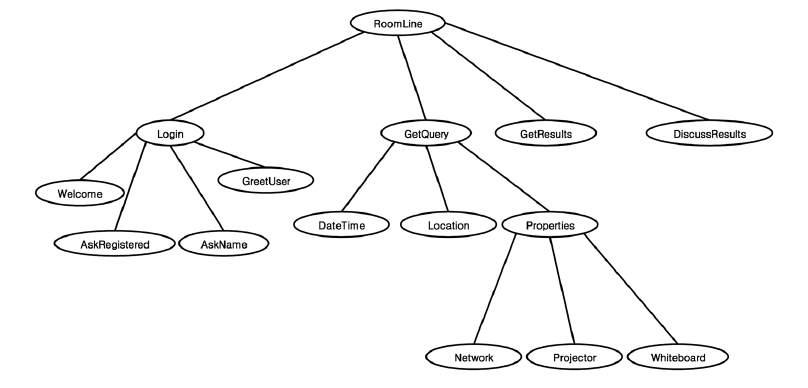
\includegraphics[width=12cm]{figures/knowledgeDM.png}
\caption{基于RavenClaw框架的RoomLine对话管理策略树}
\label{fig:knowledgeDM}
\end{figure}


\item 数据驱动的对话管理

最近几年,对话管理的研究趋势逐步转向数据驱动的方法,即通过语料库来训练相关对话结构和知识库。虽然这种数据驱动的方法需要消耗很大的时间和人力进行语料库标注,但是对话管理模型的训练几乎不需人工干涉,而且在可移植性方面,如果需要在其他领域建立一个对话系统,也只需要重新训练新的语料库,与基于知识的对话管理相比,这显然是更简便的方法。

这些优势驱动了使用无监督强化学习的随机对话建模的发展,如\cite{Levin2000}使用了基于马尔可夫决策过程(MDP)的强化学习算法,\cite{WilliamsYoung2007, Young2013, Williams2013, Kim2015, Henderson2013}使用了基于部分可观测马尔可夫决策过程(POMDP)的强化学习算法来进行对话建模。这些对话管理框架都使用数据驱动的统计机器学习算法,通过强化学习算法来优化系统的奖励或者惩罚函数,允许系统有理论原则性地根据当前的对话状态来动态修改对话策略。此外,基于POMDP的对话管理还能通过支持最优语音识别和自然语言理解结果来评估信念状态(belief state),从而达到纠正语音识别以及自然语言理解模块中出现的错误。对于基于POMDP的对话管理,系统只观测在当前状态下的有关现实世界(在对话系统中指的是语音识别和自然语言理解结果)的不完整的信息,系统必须利用当前对话状态下寻求一种最优策略将当前的信念状态映射到对话管理策略上。因此,基于POMDP的对话管理可以通过维持信念状态(即最优语音识别和自然语言理解结果)分布来实现语音识别和自然语言理解结果的纠错处理,而无需其他特殊方法。同时,有关用户的背景知识(如用户的特长以及情感状态等)也能通过可分解的强化学习模型映射到状态空间中,从而使得对话管理更人性化。

尽管强化学习算法在理论上能解决基于不确定性的推理和决策,从而为对话管理提供了有效的途径,但在实现过程中,基于强化学习的对话系统依然困难重重\cite{Paek2006},首先,对话系统中的状态包含大量语义项和项值、用户意图、理解结果和对话历史的各种可能组合,使得状态空间的规模指数增长\cite{Yukai2015},因此使得强化学习的过程计算复杂度巨大,也使得对话控制的精细改进过程变得困难;其次,强化学习得到的最优策略也剥夺了对话系统开发者对对话流程的监督指导权利。\cite{WilliamsYoung2005, Lemon2006, Young2007, Thomson2008, Williams2008b}在一定程度上对这些问题进行了改进。\cite{Lemon2006, Williams2008b}中研究了如何将传统的基于知识的对话管理和基于强化学习的对话管理结合起来构建商务领域的对话管理规则库,在一定程度上给开发人员留下了对对话管理的监督和指导的空间。然而,目前该方法仍在研究中,尚未用到实用性的对话系统中。

数据驱动的对话管理方法还包括使用最大似然估计等有监督的机器学习算法从对话语料库中训练对话模型\cite{Hurtado2005}。为了避免数据稀疏的问题,\cite{Hurtado2005}中采用了对话寄存器来表示对话状态序列用于跟踪对话历史,其中对话寄存器包含用户在整个对话历史中提供的各项信息。

基于实例的对话管理方法也是数据驱动的对话管理中的一个流行的研究方向,具有代表性的系统有\cite{Murao2003, Inui2001, Lee2009c}。该方法假定类似的对话状态会引发类似的回应,因此可以通过匹配对话实例库中的与当前对话状态最相似的对话状态来构建相应的对话模型。目前搜索与当前对话状态最相似的对话实例大多数都使用关键词来检索,对话实例库中的对话实例的表示通常采用语义约束的形式,从而整个对话实例库可以通过语义索引来概括\cite{Lee2009c}。对话管理模块首先将当前的对话状态也表示为语义约束的形式,并试图从对话实例库中找到与之相近的对话实例,如果没有返回结果,系统会放松语义约束后再一次从对话实例库中查找相近的对话实例;如果返回结果不止一个,那么系统会采用启发式算法来计算返回结果中的每一个实例与当前输入的相似度,然后选择相似度最高的返回作为应答。

数据驱动的对话管理的相关研究在近几年来发展可以说是突飞猛进,当下流行的深度机器学习也被用于对话管理领域,通过深度神经网络在大型对话语料库上训练对话模型的研究也取得了比较有前景的实验结果\cite{Shang2015, Sordoni2015b, VinyalsLe2015}。近期的相关研究还包括“端到端”的数据驱动对话管理框架,也就是利用多层次的神经网络对整个对话过程中的每一个组件以及每一个阶段都进行训练,从而得到包含从语音输入到语音输出,以及对话过程中各个阶段的一系列概率模型\cite{Serban2015}。然而,这些数据驱动的方法都严重依赖于足够大的数据集,为了取得有价值的实验结果,动辄需要上千万甚至上亿则对话。

\item 基于混合方法的对话管理

为了克服上述提到的基于知识以及数据驱动的对话管理方法中的各种不足,基于混合方法的对话管理的研究逐渐发展起来。

传统的基于强化学习的对话管理方法需要通过用户和系统的反复交互来学习一个好的对话策略,而且目前的强化学习算法的泛化能力很弱,往往需要通过大量人力去和系统交互或者庞大规模的对话语料库去归纳一个很小语境条件下的对话策略。为了解决该问题,\cite{Pietquin2006, Schatzmann2007} 中引入了用户模拟器的技术,也就是说,通过用户模拟器来代替人和对话管理器进行交互。根据有限的真实语料概括学习得到特定的用户模型,用户模拟器可产生大量的模拟对话。除此之外,\cite{Henderson2008}中还提出了将强化学习和有监督学习结合起来并在有限固定的对话语料库上学习和优化对话策略的混合方法,有监督学习的引入在一定程度降低了传统强化学习方法中对巨大对话语料库的需求程度。在该方法中,强化学习用于优化对话策略中对话奖惩的度量,而有监督学习用于指导对学习到的对话策略状态空间的剪枝,从而得到更高效有用的状态空间。

在传统的POMDP算法中,优化过程可以在任何时刻选择任意的行为,因此,没有简洁易操作的方式引入一些领域相关的常识性知识来约束和指导优化过程。例如,一个医疗相关的对话系统不应该在问病人症状之前就提供用药建议,然而,传统的POMDP算法却不存在直接的方法将该常识引入到优化过程中。近年来,也有相关研究提出来改进该问题,如\cite{Lemon2006, Williams2008b}中提出了在POMDP框架中基于传统规则来约束策略状态中的可能对话行为的集合,这样通过传统规则来对状态空间中的一些不合理的行为进行剪枝,不但加速了强化学习的优化过程,也使优化过程往更可靠的方向进行。

目前,传统的基于实例的对话管理方法应用在实用口语对话系统中还存在很多关键问题,比如先验知识的缺乏,语音识别的错误,以及语义解析的不确定性等。针对这些问题,\cite{Lee2009b}中提出了将对话实例与先验知识同时用在基于实例的对话管理中,从而提高系统的鲁棒性。该方法使用了基于议程的模型,将先验知识表示为议程图,并作为对话管理的子任务流之一来对领域相关的对话控制进行编码。这些先验知识不仅被用于预测系统的下一个对话行为,还通过议程图来跟踪对话状态,以便于处理一些话题焦点转移的意外情况。另外,该方法还通过在话语层次和语篇层次上的打分作为启发,来对当前对话状态下的N-best的对话行为假设进行重排。

基于混合方法的对话管理的最新研究趋势还包括在强化学习模型中引入概率规则的概念,\cite{Lison2015}中将概率规则定义为逻辑条件和概率事件之间的结构映射,并作为高层次的模板用于概率图模型中,其中可能包含未知参数,其值可以通过数据进行贝叶斯推断来估计得出。由于使用了逻辑的抽象化,这些概率规则可以对数据驱动的基于POMDP的对话管理中使用的概率模型进行编码成更紧凑更可读的形式。在理想情况下他们需要较少的参数估计,因此,与典型的基于POMDP的对话管理方法相比,要求较少的训练数据,也允许开发者在对话管理过程中使用人工编写的对话控制规则。然而,该方法还未成熟和完善,其实用价值在很大程度上还有待考察。

\end{enumerate}

在这些繁多的对话管理研究技术中,本文提出的方法更接近于现有技术中的通用对话建模技术,以及最新的在对话管理中引入概率规则的相关研究。然而,与这些研究又不同,本文由系统的动机出发,结合言语行为以及其他的交际行为与这些动机之间的关系来构建一个相当复杂的对话管理模型。此外,由于使用了基于概率逻辑规则的知识表示方法,本文的认知对话管理框架也能通过观测数据来进行对话模式的自适应。因此,本文的方法可以被认为是基于混合方法的对话管理。
从长远角度来看,本文提出的对话管理框架将实现以通过观测数据来进行经验概率分析为主的对话控制,不过目前,我们的研究集中于将其内置的通用对话建模将作为对话行为控制的主导。


%%%%%%%%%%%%%%%%%%%%%%%%%%%%%%%%%%%%%%%%%%%%%%%%%%%%%%%%%%%%%%%
\subsection{自然语言理解、生成研究综述}{Overview of Natural Language Understanding and Generation}
%%%%%%%%%%%%%%%%%%%%%%%%%%%%%%%%%%%%%%%%%%%%%%%%%%%%%%%%%%%%%%%

智能对话系统的研究、开发和使用都离不开自然语言理解和自然语言生成的支持,因此本小节将分别对自然语言理解和自然语言生成方面的现有研究技术以及存在的问题等进行简要的回顾。

\begin{enumerate}

\item{自然语言理解}

自然语言理解是自然语言处理(NLP)的分支领域,它是通过使用软件来理解自然语言的意义(语音,或者本文更关注的“文本”)。自然语言理解主要是将自然语言转换成抽象的语义形式,以获取语言的含义;或者是转换为某种响应(例如对某个问题的回答),以说明其理解了语言的含义。

在20世纪80年代之前,自然语言理解的方法通常是基于人工编写的复杂规则。紧随着机器学习技术的发展,基于统计的自然语言理解方法也开始兴起\cite{Tan1992}。乔姆斯基的形式语法理论以及摩尔定律使得通过语料库来进行统计学习的自然语言理解技术成为可能\cite{Gupta2014}。近些年来,越来越多的相关研究投入到无监督学习或者半监督学习方法上,这些技术能使自然语言理解不那么依靠需要大量人力获得的人工标注的语料库。一般来说,与有监督学习相比,无监督学习或者半监督学习的难度相当大\cite{Gupta2014}。

在目前主流的智能对话系统中,自然语言理解模块通常通过以下流程逐步完成:词法分析、句法分析、语义关系抽取、语义理解。词法分析主要是将字符序列转换为标记序列的过程,并非本文的研究内容,因此这里从其他几方面来介绍各流程的研究现状。


\begin{description}
\item[(1)]{句法分析}
通常自然语言理解是通过对句子的某些,或全部句法法进行分析来完成的。大量的形式化体系和算法通过特定的语法体系对句子的句法结构进行解析。大体来说,主流的句法分析包括“依存句法分析” \cite{Eisner1996a, Eisner1996b, Yamada2003} 以及 “短语结构句法分析” \cite{Chomsky1957, Pollard1994}。短语结构句法分析依据短语结构文法\cite{Thompson1981, Charniak1997, Makino1998, Charniak2006},首先对句子进行短语分析,然后指出单词和短语之间的关系,以及短语之间的关系;而依存句法分析依据依存文法\cite{Tesniere1959, Melchunk1988},仅仅在句子中的单词之间标注(有标记的)连接关系。依存句法分析是我们要在本文中探讨的语法类型。


这里的“依存”是指语言单位(如单词)由有向链接相互联系在一起。一般来说,在依存语法中,(限定)动词被视为句子或子句结构的中心,其它所有句法单位(单词)是直接或间接地与动词通过有向链接相连。这种有向链接被称为“依存”。句子结构是由一个词(中心词)与它的依存词之间的关系而决定的。


“依存”关系是一对一的对应关系:对于句子中的每个元素(例如:单词或语素)来说,实际上句子中都有一个与其相对应的节点。这种一对一的对应关系决定了“依存语法”就是单词(或语素)的语法。所有的句子都有元素和将元素组成结构的依存关系,这种情况应该与短语结构语法的“成分关系”进行比较,“成分关系”是一对一,或一对多的对应关系,也就是说,对于句子中的每个元素来说,有一个或多个与其对应的节点。这种不同带来的结果是:相比短语结构,依存结构非常紧凑,因为它往往包含很多小的节点。从计算机处理的角度来说,这种简洁的结构是有益的。


\item[(2)]{关系抽取}
自然语言理解中的一个重要方向是{\bf 关系抽取}。在NLP领域中,关系抽取已成为一个重要的研究方向,一方面是因为它的实际应用价值,另一方面因为它被看做是语义分析的一部分,而且是目前的技术相对容易实现的那部分。到目前为止,吸引最多注意力的关系抽取是命名实体之间的关系识别,例如:“个人从属关系”和“组织地址关系”。

一般来说,关系可以由一个元组的形式来定义的,$t = (e_1, e_2, ...,e_n)$。在这里,$e_i$ 是文本中预定义关系$r$ 的实体。大多数关系抽取系统主要关注二元关系的抽取。例如 :

\begin{verbatim}
位于(厦门,中国)
father-of(Richard Li, Li Ka-Shing)
\end{verbatim}

抽取“高阶关系”也非常有意义。例如这个句子:"At codons 12, the occurence of point mutations from G to T were observed'' (“在密码子12,观察到从G到T的点突变”)。句子中出现了一个4进制生物医学关系,可以描述为:

\begin{verbatim}
point mutation(codon, 12, G, T)
\end{verbatim}

目前人们普遍视“关系抽取”为一个有监督分类问题,它从一个语料库开始(语料库中包含由人类标记的相关语义关系),然后利用统计方法来对标记的关系建模,并学习出适合应用于其它文本的统计模型。

目前,关系抽取系统的主要限制在句子层面上运用。事实上,关系可能跨越句子,甚至贯穿不同的文件。然而,解决这一问题需要一定的常识和非常灵活的知识表示。本文的研究也无法直接解决这一问题,但我们相信:通过将句子意义映射为通用的知识表示,我们已经奠定了解决问题的基础。在这种知识表示中,跨句或跨文本的通用联系和推理是可以被实现的。

\item[(3)]{流结构语法}


将流结构语法(FCG)与本文使用的语言形式化体系进行比较分析是很有意义的。在FCG中,一句话语的信息是以语义和句法结构组织在一起的。语义结构是对“话语意思”的分解,它含有特定语言的语义分类,例如:“put”事项被归类为“起因-移动-位置”类事项,包括一个施事者(agent)、一个受事者(patient)和一个位置(location)。句法结构是将话语形式分解为成分和词素,还包含附加的句法分类,比如:句法特征(例如:数量和性别)、词序限制等。


从理论上来说,FCG是基于一种程序性语义的方法,在这个意义上,话语的意思是听话人假定要执行的程序,因此,概念化便是一个规划过程(规划该程序),而解析便是对该程序的执行过程。
FCG中,有关配对句法和语义结构的例子(短语“the ball”),请见图 \ref{fig:fcg1} and \ref{fig:fcg2}。

\begin{figure}[htb]
\centering
\includegraphics[width=12cm]{figures/fcg1.png}
\caption{ FCG中对短语“the ball”的句法及语义表示结构}
\label{fig:fcg1}
\end{figure}

\begin{figure}[htb]
\centering
\includegraphics[width=12cm]{figures/fcg2.png}
\caption{ FCG中对短语“the ball”的语义表示的列表形式}
\label{fig:fcg2}
\end{figure}


所有的FCG规则都是双向的。通常在产生过程中,所要表达的语义内容是与语义结构相统一的,有可能产生一组绑定。如果成功了,绑定会与语义结构相融合。这种融合可以理解为“部分统一”,但它利用结构中那些遗漏部分扩展了结构。在句法分析过程中,被分析的句子与句法结构是统一的,同时,结果中的某些部分被添加到语义结构中。
\end{description}

本文所使用的形式化体系在概念上有些类似FCG。 此外,我们有配对句法和语义结构,而且还进行双向处理。在第\ref{chap:comprehension}章中,我们将论述链语法,它将句子转换成句法结构,以及RelEx和RelEx2Logic模块,它们将句法结构转换成语义结构。在第 \ref{chap:generation}章中,我们将阐述另一个方向的Microplanner 和SuReal模块,也就是将语义结构转换成句法结构,再生成句子。本文研究的平台OpenCog中的模式匹配器(Pattern Matcher)在使用这些句法和语义结构时,也将这些结构视为有效的程序,同样实现了“程序化语义”。但我们的形式化体系与FCG的着重点不同。FCG主要是用作探索问题的理论工具,而本文的研究更侧重用于真实世界的实际应用。

\item{自然语言生成}{Natural Language Generation}

随着统计机器学习技术不断成熟和发展以及大数据的利用率不断提高,统计的方法已经被广泛用于自然语言理解的很多模块,如句法分析、语义关系抽取,甚至对话系统中的对话管理模块,并取得了很大的进展;然而,由于语义标注语料的缺乏,数据驱动的自然语言生成技术还面临着诸多困难和挑战,目前大部分自然语言生成系统仍然采用了基于规则的方法\cite{Cheyer2007, Mirkovic2011}。

自然语言生成(NLG)是自然语言理解(NLU)的反向过程。总的来说,自然语言生成是从信息的计算表示中自动生成人类(自然的)语言。由于语义知识表示体系的差异化,造成自然语言生成系统的输入多样化,因此不同的自然语言生成系统所包含的组块一般都不尽相同。概括地说,自然语言生成系统可以表示为解决下列两项任务:

\begin{itemize}
\item What should I say?(我应该说什么?)
\item How should I say it?(我应该怎么说?)
\end{itemize}

为了解决这些问题,自然语言生成系统可能涉及许多相互关联的规划模块,如:
\begin{itemize}
\item 确定要表达的信息
\item 构建语篇规划
\item 将信息块转换为语篇单位
\item 选择适当的短语和单词
\item 输出正确的语法
\end{itemize}

将这个流程分解为阶段的方法如下:
\begin{description}

\item [1)] 宏观规划

宏观规划涉及选择和组织内容。它输入的是一个或多个沟通目标:解释、描述,或提问;引起听众的某种行动或思考等。宏观规划输出的是一种知识架构,这个架构不一定是语言的属性,而是体现智能体所要沟通的信息。除了一般性内容,这种知识架构可能包含一些与沟通过程有关的信息,例如:不同的知识块应该以什么样的顺序来传达。

目前宏观规划的研究主要基于一些语篇结构层次上特定的理论体系,例如:修辞结构理论\cite{Mann1987}。在本文所介绍的研究中,我们采用了基于动机认知模型Psi的宏观规划,该模型的构建非常符合人类的心理特征。

\item [2)] 微观规划

微观规划则运用知识架构,并将它们分为句块。微观规划必须处理多种语言问题,例如:

\begin{itemize}
\item 句子范围:是否可以将两片叶子接在一起,怎样接在一起。(“我今天饿了。我去了 Burger King。” VS “我今天饿了,所以我去了Burger King。”)
\item 代词化
\item 聚合:删除重复内容。(“抽烟对你不好。抽烟会缩短你的寿命。抽烟让你口气不佳” VS “抽烟对你不好、缩短你的寿命,而且让你口气不佳”)
\item 主题化
\item 主题排序
\end{itemize}

到目前为止,大多数微观规划都是为特定的应用而专门制定的。比较典型的多用途微观规划框架如SPUD\cite{Stone1997},它利用的是一个基于逻辑的规划流程形式。尽管在细节上有所不同(原来的SPUD是基于树-邻近语法),但我们所描述的微观规划在概念上受到了SPUD的很大影响。

\item [3)] 表层生成

最后,“表面生成”涉及的是文本表层的生成,例如:把知识结构转换为句子。经典的表层生成器,例如FUF/SURGE\cite{Elhadad1992}和 Penman/KPML\cite{Matthiessen1991},都是以深层语言学理论为基础的。其他知名的系统,例如Nitrogen\cite{Langkilde1998}则采用的是统计法。所有基于规则的方法和统计法现在仍然流行。

\end{description}

\end{enumerate}

在对话系统方面的应用方面,自然语言生成的主要任务是将对话管理生成的抽象对话行为组块转换成恰当的应景的自然语言文本,通常,这里的抽象对话行为组块包含对话行为类型以及相应的(属性,值)二元组,如图\ref{fig:NLG-example-litReview}所示\cite{Wen2015}。有关这方面的研究,早期的方法有使用N-gram语言模型来对一些人工编写的语言生成器产生的可能输出结果进行重排\cite{Langkilde1998},显然该方法需要依靠大量人力来编写规则来构建语言生成器。为了减少人工编写的语言生成器的使用,\cite{Oh2000}使用基于N-gram的语言模型生成器组合来替代了这些人工编写的语言生成器,针对每一个对话类型定义一个相应的N-gram生成器,虽然\cite{Oh2000}中将人工编写的规则的使用限制在后处理的小集合上,但还是无法避免生成器产生冗余不必要的短语和句子的情况,从而使计算复杂度相当大,而且N-gram的方法也无法判断输出的结果就是包含对话行为组块中最多相关语义项的句子或文本。\cite{Mairesse2010, Mairesse2014}中提出了基于统计的以短语为生成单位的自然语言生成方法,该方法使用了统计方法在带标注的话语语料库中训练出(话语,粗糙语义概念)的二元组,从而根据抽象对话行为组块的属性值得到相关的短语或句子。该统计方法在一定程度了解决了需要大量人力来编写规则的难题,但是带语义概念标注的语料库并不成熟也很难收集,而且统计方法相对耗时,因此使得该方法很难扩展到新的领域。

\begin{figure}[htb]
\centering
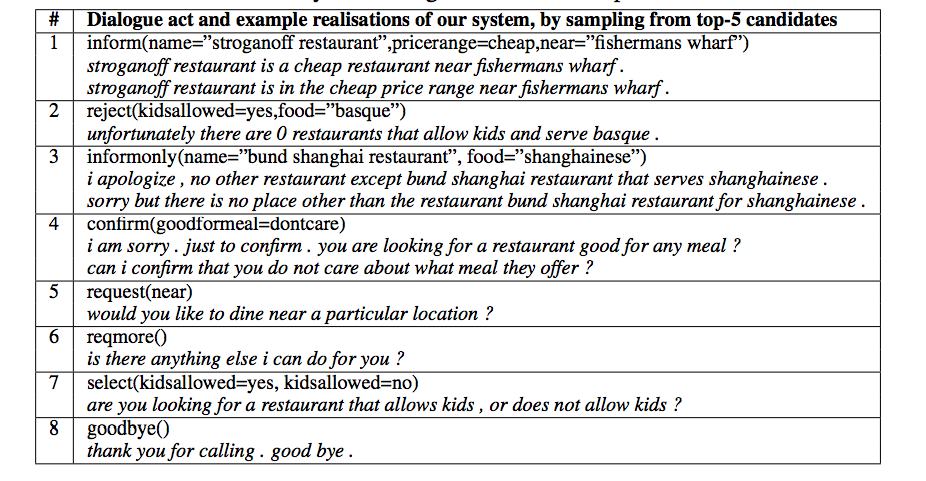
\includegraphics[width=12cm]{figures/NLG-example-litReview.png}
\caption{对话系统中自然语言生成模块的抽象对话行为实例}
\label{fig:NLG-example-litReview}
\end{figure}

针对上述这些问题,\cite{Wen2015}将深度学习的方法应用到自然语言生成领域,使用递归神经网络(RNN)和卷积神经网络(CNN)的结合来训练对话行为类型和话语的二元组。该方法无需任何的语义对齐二元组或者预先定义的语法树等标注语料库的指导,因此可以在任何领域的对话语料库上进行模型训练,使其扩展性得到了很大的提高,与上述提到的系统相比,该方法得到的实验结果也有明显的改善。但该方法只是训练出对话行为类型和话语的配对,无法用于针对抽象的语义表示形式的语言生成,然后一个好的智能对话系统中,要求的对话往往需要通过语义分析和一定的逻辑推理来生成。

总的来说,与自然语言理解相比,自然语言生成技术要落后得多。目前的实用系统往往限定在一些专业领域,而且很粗糙。概念比较先进的系统,如FCG,尚未经过广泛地实践测试。正如第\ref{chap:generation}章中所介绍的,我们在这一领域的研究代表了“基于规则的方法”和“统计法”的融合。我们认为这种融合非常有前景,但目前还没有精细化,也没有经过系统性评估。

%%%%%%%%%%%%%%%%%%%%%%%%%%%%%%%%%%%%%%%%%%%%%%%%%%%%%%%%%%%%%%%
\subsection{言语行为理论及相关研究综述}{Overview of Speech Act Theory and related research}
\label{sec:speechAct}
%%%%%%%%%%%%%%%%%%%%%%%%%%%%%%%%%%%%%%%%%%%%%%%%%%%%%%%%%%%%%%%

我们认为,分析和管理对话系统需要产生的各类话语的一个有效方法是:使用由Austin\cite{Austin2005}提出,Searle\cite{Searle1969} 改进的言语行为理论(Speech Act Theory)。本文将要阐述的智能对话研究中正采用了此方法,且在研究过程中,我们发现这个理论是极其有用且方便使用的。我们在这一节先回顾言语行为理论的基本观点,并介绍一些言语行为理论在对话方面的相关研究以及更细致具体的分类体系。

言语行为理论是语言学和语用学等研究中的一个重要理论。言语行为理论的核心概念是:强调语言的意向功能,认为说话者在说话的同时是在实施某种行为。因此,根据言语行为的观点,分析说话者的语言行为的过程,也就是说话者分析为了实现某个特定目标而采用的一系列的言语行为的过程。

言语行为理论探讨那些可以通过言语来表现的行为类型。Austin\cite{Austin2005}将言语行为分为以下几种:

\begin{itemize}
\item {\bf 言内行为(Locutionary Act)}:话语的外在表现形式,即:话语本身的字面意义。
\item {\bf 言外行为(Illocutionary Act)}:话语的“言外之力”,即:说话者对受话者的影响。
\item {\bf 言后行为(Perlocutionary Act)}:话语达到的实际效果,即:话语所导致的行为,如说服、劝说、吓唬、启发、激励,或者让受话者去做某件事,或者让受话者意识到什么,不论是有意还是无意的。
\end{itemize}

Searle对Austin提出的言语行为理论做了深入的研究和探讨。在Searle\cite{Searle1969}看来,言语行为有时仅仅指的是言外行为。他认为,说话人通过他们的言语只能获得5类言外之力,它们分别是:

\begin{itemize}
\item 断言类:说话人自己承诺事情是真的。The sky is blue. (天是蓝色的。)
\item 指令类:说话人试图让受话人做某事。Clean your room! (打扫你的房间!)
\item 承诺类:说话人对未来的行为做出承诺。I will do it. (我将会做这件事。)
\item 表达类:说话者表达了某些心理状态。I’m Sorry. (对不起。)。
\item 声明类:说话人带来了不同的状况。The meeting is adjourned.(这个会议休会了。)
\end{itemize}

受这个本体论的启发,Twitchell 和 Nunamake在他们2004年的论文(标题为:言语行为归档:分析持续谈话和其参与者的概率统计法。\cite{Twitchell2004})中提出了更加精细的“42种言语行为”本体论,叫做SWBD-DAMSL (DAMSL = Dialogue Act Markup in Several Layers)。尽管有少量不符合Searle的观点,并被分类为“其它”,但几乎他们所有的42种言语行为类型都能够被映射到Searle的5个高级类别之一。图\ref{fig:DAMSL}和\ref{fig:Searle}描述了这42种行为和它们与Searle分类之间的关系。我们已经利用了这个Searle解析法,它给我们正在进行的自然语言对话研究带来了灵感。

\begin{figure}[htb]
\centering
\includegraphics[width=12cm]{figures/DAMSL.png}
\caption{SWBD-DAMSL中使用的42种言语行为}
\label{fig:DAMSL}
\end{figure}

\begin{figure}[htb]
\centering
\includegraphics[width=12cm]{figures/Searle.png}
\caption{ 42种SWBD-DAMSL言语行为类型与Searle的言语行为类型的关联}
\label{fig:Searle}
\end{figure}


总之,言语行为理论为对话管理和对话控制提供了一个新的思路,也就是将对话的话语看成是一种行为,这样不仅能通过对不同言语行为的定义来猜测说话人的意图,还能将对话行为看成和其他非语言的行为类似。不难看出,它不仅给对话管理和对话控制提供更多可行的用于非语言的行为控制机制,也同时能将对话与智能体的其他行为有效结合起来,从而完成更智能更人性化的对话。

%%%%%%%%%%%%%%%%%%%%%%%%%%%%%%%%%%%%%%%%%%%%%%%%%%%%%%%%%%%%%%%
\section{存在的问题}{Omissions of Present Research}
%%%%%%%%%%%%%%%%%%%%%%%%%%%%%%%%%%%%%%%%%%%%%%%%%%%%%%%%%%%%%%%

对话系统的研究已有几十年的历史,尽管有不少学者,这些对话系统能够满足一些娱乐性的需求和非常限定场合下的信息查询用途,但仍有许多亟待改进的地方,主要包括:

(1)知识深层表示问题

        认知对话系统首先需要一个能存储丰富语义信息且能灵活操作的深层语义表示体系来支撑,这样一来,对话系统就能从自然语言话语中捕获浅层的句法信息之外的深层语义信息,用于指导对话系统的认知过程。 然而知识表示体系的研究面临着表达能力和计算效率两大挑战,目前很多知识表示体系不得不为了使计算效率达到可用范围而牺牲其表达能力,也就是说,只能表达小规模的知识,一旦知识库达到一定规模,往往出现很多不可操控的问题。

(2)不确定性逻辑推理问题

       不少对话系统中不考虑非精确条件下的语言理解问题,以及在不确定的条件下对话系统如何推断和决策问题。我们认为,具有认知功能的对话过程不仅需要具备一定的逻辑推理功能,即通过演绎、归纳和回溯等推理过程实现的推理,还需要具备不确定推理功能,即涉及概率和模糊逻辑等不确定性的推理,从而使得对话系统能允许非精确输入,并实现在非精确条件下的有效理解,提高对话交互的自然度。

(3)语言和涉身知识的融合问题

       目前的对话系统基本上只考虑语言层面上的交互,但是,自然的对话交流都需要考虑特定的语境和语用等方面的信息,语言的交互也不仅仅是语言层面上的交互,还需要理解语言背后涉及到的涉身交互,也就是说,每一句话语应该被理解成一个“言语行为”,即包含一些独特的语言属性,还包含一些涉及到言语行为和其他类型行为的语用属性,也就是通常所说“言外之意”。

(4)动机驱动的对话控制:

     大多数对话系统都是作为一个执行主体来完成用户指派的对话任务,然而要实现自然的对话交互,还要求机器能作为一个认知主体,能去适应人的交流方式。我们认为,认知对话系统应该根据智能体本身的动机来做决策,并且能在交互的过程中根据人的方式来调整系统动机,以实现更拟人更逼真的对话。也就是说,对话系统在决定什么时候说什么时,必须有一个动机驱动的行为选择模型来指导,而不是基于简单的浅层语言提示来进行回应。


%%%%%%%%%%%%%%%%%%%%%%%%%%%%%%%%%%%%%%%%%%%%%%%%%%%%%%%%%%%%%%%
\section{研究目标和内容}{Goals and Contributions}
%%%%%%%%%%%%%%%%%%%%%%%%%%%%%%%%%%%%%%%%%%%%%%%%%%%%%%%%%%%%%%%

构建一个能达到人类水平的对话系统是一项十分艰巨的任务,实现这个长远目标远超过本文所能涵盖的范围。本文针对当前相关研究存在的问题,提出了本课题的研究目标:从对话系统的认知需求着手,深入研究知识表示的深层模型以及在该表示上的不确定概率推理,设计并实现自然语言理解和自然语言生成的流程,实现架构从语言到逻辑之间的桥梁。采取动机驱动的情感计算模型和言语行为理论的思想指导,提出一个能使对话系统具有一定认知能力的动机驱动的对话控制模型;并在该模型上实现一个以信息查询为动机的问答系统。

       本文的主要研究内容如下:
(1)研究对话系统的认知需求,借鉴心理学动机模型、言语行为理论以及概率逻辑推理理论等,提出一个动机驱动的对话控制模型。

(2)研究知识的深层表示问题,使其不但能有效储存丰富的语义语境信息,还能被灵活操作。

(3)研究基于深层知识表示的自然语言理解机制,设计并实现一个自然语言理解框架,使其能将自然语言语句转换成(2)中使用的基于超图的抽象的逻辑语义表示形式。

(4)研究基于深层知识表示的自然语言生成机制,设计并实现一个自然语言生成框架,使其能将基于(2)的深层表示的抽象逻辑语义形式转换成自然语言语句。

(5)研究不确定性逻辑推理,将概率逻辑网络应用在深层知识表示结构中,设计和实现一个能在自然语言语句上执行的常识推理系统。

(6)借助上述(3)中的自然语言理解框架,将简单的英文维基百科进行自然语言理解处理并表示成基于超图的深层语义表示形式,并在(1)中的对话控制模型上实现一个以信息查询为动机的问答系统。

%%%%%%%%%%%%%%%%%%%%%%%%%%%%%%%%%%%%%%%%%%%%%%%%%%%%%%%%%%%%%%%
\section{论文的组织结构}{Outline}
%%%%%%%%%%%%%%%%%%%%%%%%%%%%%%%%%%%%%%%%%%%%%%%%%%%%%%%%%%%%%%%

本文按照如下方式组织:

第一章,给出了认知对话系统的研究背景和意义,总结了国内外相关领域的研究现状,并指出了现有研究的局限和存在的问题。最后,给出了本文的研究目标,并介绍了本文的主要研究内容。

第二章,深入探讨了认知对话系统中所使用的深层知识表示体系,并从范畴论角度出发,阐述了能将自然语言映射到该表示体系的理论基础,最后,我们还介绍了能用在该表示体系上不确定性逻辑推理机制,即概率逻辑网。

第三章,主要介绍了动机驱动的情感计算模型Psi,以及该模型中所采用的情感和人性等机制,为下一章节的动机驱动的对话控制模型提供一定的背景知识和理论基础。

第四章,本章首先讨论了如何对心理学上动机驱动的情感计算模型Psi进行改进,使其能用在本文的认知对话控制机制中,然后介绍了认知对话系统的相关目标和动机,提出了引入逻辑推理的动机驱动的行为控制策略,并提出了使用动机驱动来进行对话语篇管理;结合言语行为理论,针对不同的言语行为类型提出了不同的言语行为规划器;最后,结合上述研究成果,提出了动机驱动的对话控制模型。

第五章,介绍本文设计实现的将语言转换成超图表示的抽象逻辑形式的自然语言理解流程框架,借助链语法输出的链集合,将其映射到使用超图来表示的更抽象的逻辑关系集合。

第六章,介绍本文设计实现的将超图表示的抽象逻辑形式转换自然语言语句的自然语言生成流程框架,通过微观规划器来重新组织和整理超图表示的抽象逻辑关系,并利用基于超图匹配的表层生成器将这些整理后的抽象逻辑关系转换成自然语言语句。

第七章,介绍本文设计的对自然语言语句进行逻辑推理的机制,结合本文设计和实现的自然语言理解框架,将自然语言语句转换成超图形式表示的抽象逻辑关系集合,并使用概率逻辑网络进行推理,最终将推理后得到的超图表示的逻辑关系集合转换成自然语言语句的形式,特别给出了对带比较级的句子进行推理的过程。

第八章,结合第五、六、七章的研究成果,将简单的英语维基百科上的知识表示成第二章中的超图形式,并在第四章的动机驱动的对话控制模型上,设计并实现了一个以信息查询为动机的基于概率逻辑推理的问答系统。

第九章,对全篇论文的研究进行总结,列出本文的主要贡献和创新点,并提出下一步的研究方向和对未来研究的展望。
